    \subsection{Accuracy (backward stability)}
    \paragraph{Metric.}
    We define the following metrics in order to test backward stability:
    \begin{align} 
        res_A &= \frac{\Vert U^TAQ - CR\Vert_1}{max(m,n)\Vert A \Vert_1 \epsilon}  \\[0.8em]  \label{backward_error_1}
        res_b &= \frac{\Vert V^TBQ - SR\Vert_1}{max(p,n)\Vert B \Vert_1 \epsilon}  \\[0.8em]  
        orth_U &= \frac{\Vert I - U^TU\Vert_1}{m \epsilon} \\[0.8em]  
        orth_V &= \frac{\Vert I - V^TV\Vert_1}{p \epsilon} \\[0.8em]  
        orth_Q &= \frac{\Vert I - Q^TQ\Vert_1}{n \epsilon} \label{backward_error_5}
    \end{align}
    where $\epsilon$ is machine precision of input data type.
    
    \subsubsection{Numerical examples of small matrices}

    We also record the stability metrics computed by both versions in Julia in Table \ref{tab:sta_test_1}.
        \begin{table}[H]
        \centering
        \begin{tabular}{||c | c || c | c | c | c | c||} 
         \hline
         & Version & $res_A$ & $res_B$ & $orth_U$ & $orth_V$ & $orth_Q$ \\ [0.5ex] 
         \hline\hline
         \multirow{2}{5em}{Example 1} & proposed & 0.2956 & 0.5646 & 0.5308 & 1.0417 & 1.1790 \\ 
         & Julia 1.3 & 0.3599 & 0.4571 & 0.9117 & 1.7083 & 1.3250 \\
        \hline\hline
        \multirow{2}{5em}{Example 2} & proposed & 0.6173 & 0.4098 & 1.5000 & 0.5613 & 1.3998 \\ 
         & Julia 1.3 & 0.5068 & 0.5689 & 1.4583 & 0.9245 & 1.2483 \\
        \hline\hline
        \multirow{2}{5em}{Example 3} & proposed & 0.4181 & 0.8941 & 0.7500 & 1.3940 & 1.3277 \\ 
         & Julia 1.3 & 0.3536 & 0.5938 & 1.4791 & 1.9540 & 1.1062\\
        \hline\hline
        \multirow{2}{5em}{Example 4} & proposed & 0.3600 & 0.5900 & 0.6558 & 0.5385 & 1.4362 \\ 
         & Julia 1.3 & 0.4449 & 0.3056 & 1.3225 & 0.7205 & 1.1814 \\
        \hline\hline
        \end{tabular}
        \caption{Stability profiling for small matrices}
        \label{tab:sta_test_1}
        \end{table}
        
    \subsubsection{Random dense matrices}
        \paragraph{Test matrix generation.} As discussed in Section \ref{def}, we test stability on four cases depending on the row and column size of the input matrix pair. In this section, we test random dense matrices of \texttt{Float64}. For each case, we choose four subcases from low to high matrix size. We generate a total of 320 random matrix pairs, 20 for each subcase.
        
        \paragraph{Results.}
        As a demonstration, we list the results of five stability metrics for each subcase of a single test run in Table \ref{tab: sta_test_2}. All 320 test runs yield results no greater than two. 
    \newpage 
    
    \begin{table}[!htbp]
        \centering
        \begin{tabular}{||c | c | c | c | c || c | c | c | c | c||} 
         \hline
         & $m$ & $p$ & $n$ & $k+l$ & $res_A$ & $res_B$ & $orth_U$ & $orth_V$ & $orth_Q$ \\ [0.5ex] 
         \hline\hline
         \multirow{4}{5em}{$m \geq n$ \\ $p \geq n$} & 60 & 50 & 40 & 40 & 0.1607 & 0.2710 & 0.7924 & 1.0079 & 0.4609 \\
         & 300 & 250 & 200 & 200 & 0.0369 & 0.0484 & 0.5041 & 0.6408 & 0.3202 \\
         & 900 & 750 & 600 & 600 & 0.0181 & 0.0193 & 0.3952 & 0.5157 & 0.2307 \\
         & 1500 & 1250 & 1000 & 1000 & 0.0120 & 0.0142 & 0.3702 & 0.4129 & 0.1847 \\
        \hline\hline
         \multirow{4}{5em}{$m \geq n > p$} & 60 & 40 & 50 & 50 & 0.1529 & 0.2261 & 0.7653 & 1.1960 & 0.6074 \\
         & 300 & 200 & 250 & 250 & 0.0412 & 0.0620 & 0.5559 & 0.7492 & 0.3150 \\
         & 900 & 600 & 750 & 750 & 0.0169 & 0.0232 & 0.4174 & 0.5250 & 0.2411 \\
         & 1500 & 1000 & 1250 & 1250 & 0.0122 & 0.0160 & 0.3726 & 0.4723 & 0.2080 \\
         \hline\hline 
         \multirow{4}{5em}{$p \geq n > m$} & 40 & 60 & 50 & 50 & 0.1672 & 0.2028 & 1.1293 & 0.9373  & 0.4217\\
         & 200 & 300 & 250 & 250 & 0.0595 & 0.0530 & 0.7064 & 0.5855 &  0.3065 \\
         & 600 & 900 & 750 & 750 & 0.0231 & 0.0231 & 0.5178 & 0.4186 & 0.2112 \\
         & 1000 & 1500 & 1250 & 1250 & 0.0164 & 0.0153 & 0.4543 & 0.3673 & 0.1778 \\
         \hline \hline
         \multirow{4}{5em}{$n > m$\\ $n > p$ } & 20 & 30 & 60 & 50 & 0.0483 & 0.0464 & 0.5472 & 0.5358 & 0.4547\\
         & 200 & 300 & 600 & 500 & 0.0120 & 0.0105 & 0.3036 & 0.3030 & 0.2374 \\
         & 400 & 600 & 1200 & 1000 & 0.0081 & 0.0072 & 0.2888 & 0.2813 & 0.2315\\
         & 1000 & 1500 & 3000 & 2500 & 0.0053 & 0.0047 & 0.2700 & 0.2605 & 0.2410 \\
         \hline
        \end{tabular}
        \caption{Stability profiling for random dense matrices}
        \label{tab: sta_test_2}
        \end{table}
    
    \subsubsection{Special types of matrices}
        
    \newpage
    \subsection{Timing}
        We want to evaluate the timing performance of our implementation between current version in Julia and MATLAB. 
        
        \paragraph{vs. Julia 1.3}
        For the comparison with Julia 1.3, we also spilt into four cases. Each case, we calculated the average CPU timing of 10 runs. In all cases, we can see that the speedup is exponential when input size is greater than a few hundreds. 
        
        \begin{figure}[H]
            \centering
            \begin{minipage}{.65\textwidth}
              \centering
              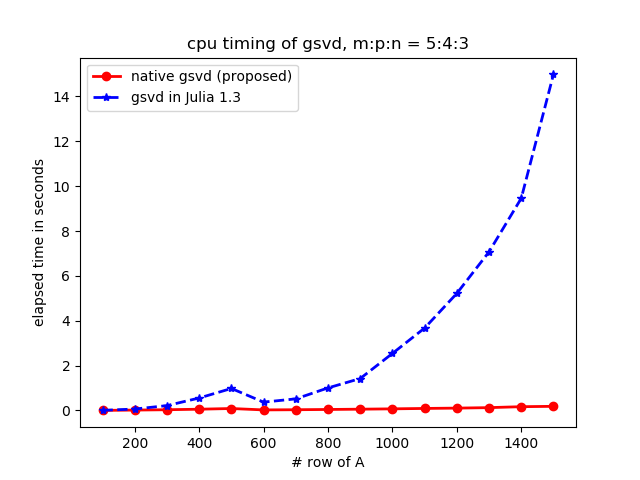
\includegraphics[width=\linewidth]{fig/m p n 5 4 3.png}
            \end{minipage}%
        \end{figure}
        
        \begin{figure}[H]
            \centering
            \begin{minipage}{.65\textwidth}
              \centering
              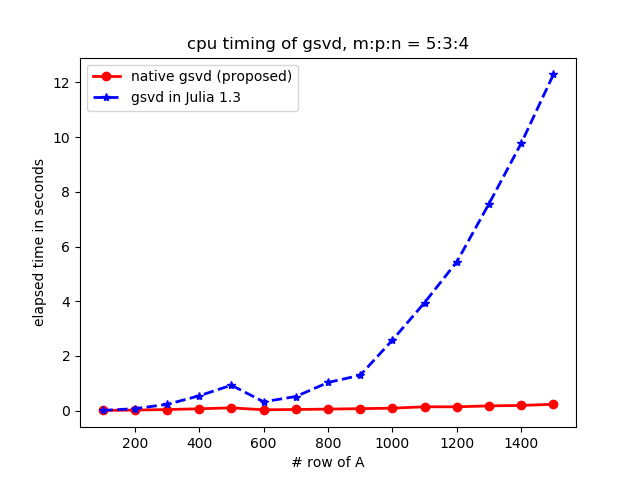
\includegraphics[width=\linewidth]{fig/m p n 5 3 4.png}
            \end{minipage}
            \label{cur_new_1}
        \end{figure}
    
        \begin{figure}[H]
            \centering
            \begin{minipage}{.65\textwidth}
              \centering
              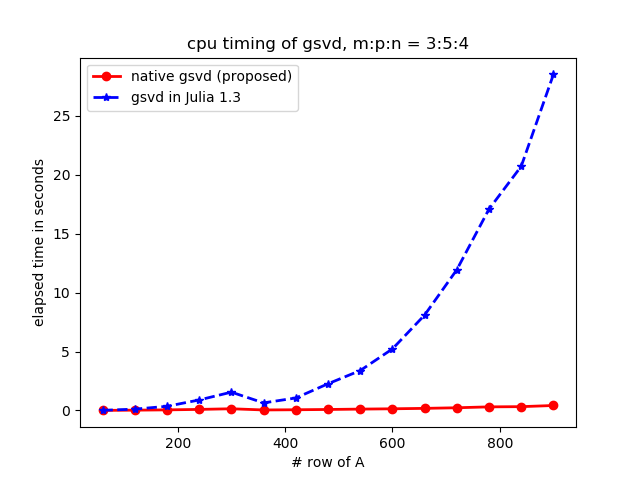
\includegraphics[width=\linewidth]{fig/m p n 3 5 4.png}
            \end{minipage}%
            
        \end{figure}
        
        \begin{figure}[H]
            \centering
            \begin{minipage}{.65\textwidth}
              \centering
              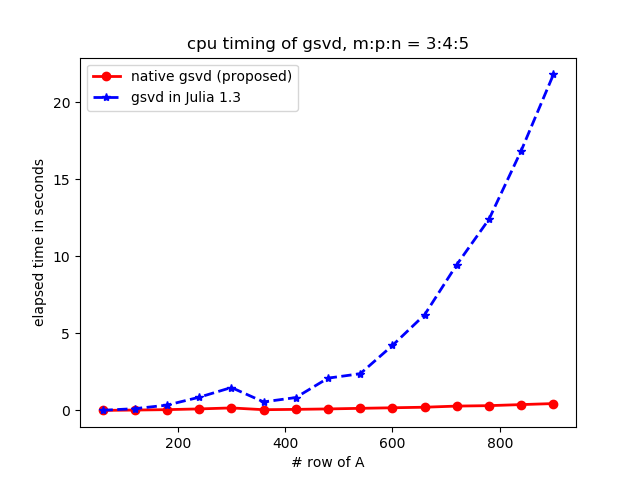
\includegraphics[width=\linewidth]{fig/m p n 3 4 5.png}
            \end{minipage}
            \label{cur_new_2}
        \end{figure}
        
        \paragraph{vs. MATLAB.}
        For the comparison with MATLAB 2019b, we specify the input as square matrix. Our implementation is still slower than MATLAB. The major reason is due to the significant difference of decomposition discussed in \ref{def} and \ref{def_mat}. 
        
        \begin{figure}[H]
            \centering
            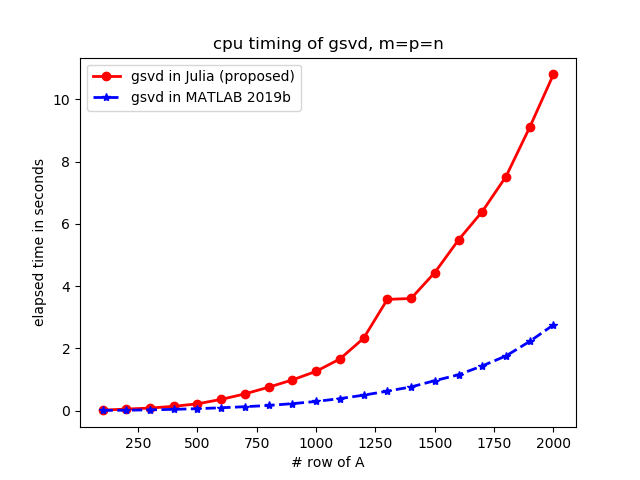
\includegraphics[width=0.65\linewidth]{fig/Julia VS MATLAB m=n=p.png}
            \label{julia_matlab}
        \end{figure}
    
    \newpage
    
    \paragraph{Profile.}
    As detailed in \ref{alg}, our algorithm insists of four parts: pre-processing, QR, CSD and post-processing. Here, we measure the CPU time spent in the first three parts and total time, denoted as $t_{pre}, t_{qr}, t_{csd}$ and   $t_{all}$ and calculated the percentages that each part spent to total time, denoted as $p_{pre}, p_{qr}, p_{csd}$. Still, we separate our test into four cases and record the average of 10 test runs. \textcolor{red}{In most cases, pre-processing dominates the computation effort}. This motivates us to explore time profiling of pre-processing. 
    
    \begin{center}
        \begin{table}[H]
        \begin{tabular}{||c | c | c | c || c | c | c | c | c | c | c ||} 
         \hline
          & $m$ & $p$ & $n$ & $t_{pre}$ & $p_{pre}$ & $t_{qr}$ & $p_{qr}$ & $t_{csd}$ & $p_{csd}$ & $t_{all}$ \\ [0.5ex] 
         \hline\hline
         \multirow{4}{5em}{$m \geq n$ \\ $p \geq n$} & 1500 & 1200 & 1000 & 0.6242 & 41.13\% & 0.1683 & 11.09\% & 0.6011 & 39.61\% & 1.5175\\
         & 500 & 500 & 500 & 0.0651 & 26.78\% &  0.0347 & 14.29\% & 0.1191 & 48.94\% & 0.2433 \\
         & 650 & 310 & 230 & 0.0418 & 54.63\% & 0.0084 & 11.08\% & 0.0195 & 25.47\% & 0.0766 \\
         & 430 & 610 & 210 & 0.0345 & 47.65\% & 0.0067 & 9.25\% & 0.0247 & 34.11\% & 0.0725 \\
        \hline\hline
         \multirow{4}{5em}{$m \geq n > p$} & 1500 & 1000 & 1200 & 1.500 & 60.09\% & 0.1815 & 7.27\% & 0.6811 & 27.28\% & 2.4963 \\ 
         & 720 & 220 & 540 & 0.1182 & 73.65\% & 0.0074 & 4.61\% & 0.0256 & 15.94\% & 0.1605 \\
         & 440 & 180 & 440 & 0.0651 & 65.84\% & 0.0053 & 5.37\% & 0.0221 & 22.41\% & 0.0989 \\
         & 370 & 290 & 350 & 0.0659 & 51.61\% & 0.0123 & 9.65\% & 0.0400 & 31.34\% & 0.1278 \\
         \hline\hline 
         \multirow{4}{5em}{$p \geq n > m$} & 1000 & 1500 & 1200 & 0.5234 & 23.23\% & 0.2789 & 12.37\% & 1.2630 & 56.06\% & 2.2529 \\
         & 250 & 300 & 300 & 0.0205 & 24.96\% & 0.0129 & 15.75\% & 0.0397 & 48.25\% & 0.0822 \\
         & 360 & 660 & 600 & 0.0645 & 18.33\% & 0.0436 & 12.39\% & 0.2103 & 59.72\% & 0.3521 \\
         & 130 & 520 & 480 & 0.0311 & 14.52\% & 0.0215 & 10.02\% & 0.1391 & 64.79\% & 0.2146 \\
         \hline \hline
         \multirow{4}{5em}{$n > m$\\ $n > p$} & 1000 & 1200 & 1500 & 1.7532 & 48.51\% & 0.2038 & 5.64\% & 1.4467 &  40.03\% & 3.6136\\
         & 260 & 600 & 770 & 0.2791 & 38.86\% & 0.0441 & 6.14\% & 0.3459 & 48.17\% & 0.7181 \\
         & 370 & 250 & 700 & 0.1385 & 86.69\% & 0 & 0\% & 0 & 0\% & 0.1598\\
         & 120 & 120 & 400 & 0.0296 & 96.70\% & 0 & 0\% & 0 & 0\% & 0.0307\\
         \hline
        \end{tabular}
        \caption{Time profiling for GSVD}
        \label{table:2}
        \end{table}
        \end{center}
        
        \newpage
    
    \paragraph{Pre-processing.}To avoid skipping steps in pre-processing, we use rank-deficient matrix as input of $B$. Likewise the time profiling of GSVD, we record absolute time spent in each part and the relative percentage to total time. The meaning of subscript in Table \ref{table:3} is explained below:
    \begin{enumerate}
        \item $qrpB$: QR decomposition with column pivoting of $B$.
        \item $genV$: Generate $V$.
        \item $updateA1st$: First time to update $A$.
        \item $genQ$: Geneate $Q$.
        \item $rqB$: RQ decomposition of $B$.
        \item $updateA2nd$: Second time to update $A$.
        \item $updateQ1st$: First time to update $Q$.
        \item $qrpA$: QR decomposition with column pivoting of $A$.
        \item $genU$: Generate $U$.
        \item $updateA3rd$: Third time to update $A$.
        \item $updateQ2nd$: Second time to update $Q$.
        \item $rqA$: RQ decomposition of $A$.
        \item $updateQ3rd$: Third time to update $Q$.
        \item $qrA$: QR decomposition of $A$.
        \item $updateU$: Update $U$.
    \end{enumerate}
    
    \newpage
    
    \begin{table}[H]
        \centering 
        \resizebox{0.8\columnwidth}{!}{%

        \begin{tabular}{||c | c | c | c ||} 
         \hline
            & \makecell{$m = 1200, p = 1000, n = 900$ \\ $l = 800, k = 100$} & \makecell{$m = 500, p = 500, n = 600$ \\ $l = 400, k = 200$} & \makecell{$m = 250, p = 200, n = 200$ \\ $l = 150, k = 50$} \\ [0.5ex]
        \hline
          $t_{qrpB}$ ($p$-by-$n$) & 0.036821 &  0.018432 & 0.002894 \\ [0.5ex] \hline
          $p_{qrpB}$ & 15.29\% &  21.59\% & 11.19\% \\ [0.5ex] \hline
          $t_{genV}$ ($p$-by-$p$) & 0.022350 &  0.006850 & 0.001578 \\ [0.5ex] \hline
          $p_{genV}$ & 9.28\% &  8.02\% & 6.10\% \\ [0.5ex] \hline
          $t_{updateA1st}$ ($m$-by-$n$) & 0.012765 & 0.005162 & 0.000736 \\ [0.5ex] \hline
          $p_{updateA1st}$ & 5.30\% & 6.05\% & 2.84\% \\ [0.5ex] \hline
          $t_{genQ}$ ($n$-by-$n$) & 0.002553 & 0.001187 & 0.000195 \\ [0.5ex] \hline
          $p_{genQ}$ & 1.06\% & 1.39\% & 0.75\% \\ [0.5ex]
        \hline\hline
        
          $t_{rqB}$ ($l$-by-$n$) & 0.024456 & 0.010305 & 0.001856 \\ [0.5ex] \hline
          $p_{rqB}$ & 10.16\% & 12.07\% & 7.18\% \\ [0.5ex] \hline
          $t_{updateA2nd}$ ($m$-by-$n$) & 0.019261 & 0.005071 & 0.000781 \\ [0.5ex]\hline
          $p_{updateA2nd}$ & 8.00\% & 5.94\% & 3.02\% \\ [0.5ex]\hline
          $t_{updateQ1st}$ ($n$-by-$n$) & 0.014279 & 0.005488 & 0.000732 \\ [0.5ex]\hline
          $p_{updateQ1st}$ & 5.93\% & 6.43\% & 2.82\% \\ [0.5ex]
         \hline\hline
         
          $t_{qrpA}$ ($m$-by-$n-l$) & 0.002878 & 0.004063 & 0.000595 \\ [0.5ex] \hline
          $p_{qrpA}$ & 1.20\% & 4.76\% & 2.30\% \\ [0.5ex] \hline
          $t_{genU}$ ($m$-by-$m$) & 0.015431 & 0.007718 & 0.001051 \\ [0.5ex]\hline
          $p_{genU}$ & 6.40\% & 9.04\% & 4.06\% \\ [0.5ex]\hline
          $t_{updateA3rd}$ ($m$-by-$l$)& 0.009105 & 0.002531 & 0.000412 \\ [0.5ex]\hline
          $p_{updateA3rd}$ & 3.78\% & 2.96\% & 1.59\% \\ [0.5ex]\hline
          $t_{updateQ2nd}$ ($n$-by-$n-l$)& 0.000289 & 0.000871 & 0.000136 \\ [0.5ex]\hline
          $p_{updateQ2nd}$ & 0.12\% & 1.02\% & 0.53\% \\ [0.5ex]\hline
          \hline
         
          $t_{rqA}$ ($k$-by-$n-l$) & 0 & 0 & 0 \\ [0.5ex] \hline
          $p_{rqA}$ & 0\% & 0\% & 0\% \\ [0.5ex] \hline
          $t_{updateQ3rd}$ ($n$-by-$n-l$)& 0 & 0 & 0 \\ [0.5ex]\hline
          $p_{updateQ3rd}$ & 0\% & 0\% & 0\% \\ [0.5ex]
          \hline\hline
          
          $t_{qrA}$ ($m-k$-by-$l$) & 0.022391 & 0.002823 & 0.001756 \\ [0.5ex] \hline
          $p_{qrA}$ & 9.30\% & 4.76\% & 6.79\% \\ [0.5ex] \hline
          $t_{updateU}$ ($m$-by-$m-k$)& 0.022113 & 0.001799 & 0.000850 \\ [0.5ex]\hline
          $p_{updateU}$ & 9.18\% & 2.11\% & 3.28\% \\ [0.5ex]
          \hline\hline
          $t_{all}$ & 0.240752 & 0.085373 & 0.025867 \\[0.5ex]
          \hline
        \end{tabular}
        }
        \caption{Time profiling for Preprocessing}
    \label{table:3}
    \end{table}
